\documentclass[12pt, twoside]{article}
\usepackage[letterpaper, margin=1in, head=30pt, headsep=0.1in]{geometry}
\usepackage[english]{babel}
\usepackage[utf8]{inputenc}
\usepackage{amsmath}
\usepackage{amsfonts}
\usepackage{amssymb}
\usepackage{tikz}
\usetikzlibrary{quotes, angles}

\usepackage{graphicx}
\usepackage{enumitem}
\usepackage{multicol}

%\usepackage{pgfplots}
%\pgfplotsset{width=10cm,compat=1.9}
%\usepgfplotslibrary{statistics}
%\usepackage{pgfplotstable}
%\usepackage{tkz-fct}
%\usepackage{venndiagram}

\usepackage{fancyhdr}
\pagestyle{fancy}
\fancyhf{}
\renewcommand{\headrulewidth}{0pt} % disable the underline of the header
\raggedbottom
\newif\ifmeta
\metatrue %print standards and topics tags

\title{Math AI Worksheet Generator and Formative Assessment System}
\author{Chris Huson}
\date{January 2021}

%\fancyhead[RE]{\thepage}
%\fancyhead[RO]{\thepage \\ Name: \hspace{3cm}}
%\fancyhead[L]{BECA / Dr. Huson / 10th Grade Geometry\\* 7 June 2019}
%
%\begin{document}
%\subsubsection*{13.7 Homework: Cross sections, distance applications}
%\fancyhead[L]{BECA / Dr. Huson / Geometry 03-Volume+angle-bisectors\\* pset ID: 34}

\begin{document}

\subsubsection*{5.9 Prequiz: Transformations}
\begin{enumerate}

\item A $110^\circ$ counterclockwise rotation centered at $P$ maps triangle $CAT$ onto triangle $DOG$. \\[0.5cm]
Write the letter or letters for each corresponding object. \vspace{0.5cm}
  \begin{multicols}{2}
    \begin{tikzpicture}[scale=1.4, rotate=20]
      \coordinate [label=above left:$D$](A) at (65:2);
      \coordinate [label=below right:$O$](B) at (1, 0);
      \coordinate [label=right:$G$](C) at (15:3.5);
      \draw [thick] (A)--(B)--(C)--cycle;
      \draw [thick, rotate=-110] (65:2) node[right]{$C$}--
      (1,0) node[below left]{$A$}--
      (15:3.5) node[right]{$T$}--cycle;
      \draw [fill] (0,0) circle [radius=0.05] node[left] {$P$};
      \draw [dashed] (0,0) circle [radius=1];
    \end{tikzpicture}

    \begin{enumerate}
      \item $T \rightarrow$ \vspace{1.5cm}
      \item $A \rightarrow$ \vspace{1.5cm}
      \item $AC \rightarrow$ \vspace{1.5cm}
    \end{enumerate}
  \end{multicols}

\newpage
\item A translation maps $A$ to $A'$, as shown, $A(6,5) \rightarrow A'(2,2)$.
\begin{multicols}{2}
  \begin{enumerate}
    \item Apply the same translation to $C(7,2)\rightarrow C'(x,y)$ on the grid. Mark and label point $C'$ as an ordered pair.
    \item Which direction is the slide?
    \begin{enumerate}[label=(\Alph*)]
      \item Up, to the right
      \item Up, to the left
      \item Down, to the right
      \item Down, to the left
      \item None of the above
    \end{enumerate} \vspace{2cm}

    \end{enumerate}
    \begin{flushright}
    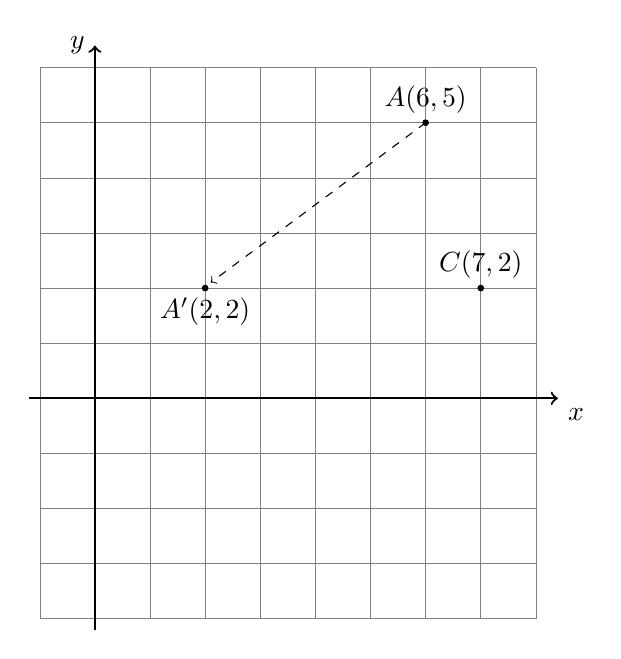
\begin{tikzpicture}[scale=0.7]
      \draw [help lines] (-1,-4) grid (8,6);
      \draw [thick, ->] (-1.2,0) -- (8.4,0) node [below right] {$x$};
      \draw [thick, ->] (0,-4.2)--(0,6.4) node [left] {$y$};
      \draw [fill] (6,5) circle [radius=0.05] node[above] {$A(6,5)$};
      \draw [fill] (2,2) circle [radius=0.05] node[below] {$A'(2,2)$};
      \draw [->, dashed] (6,5)--(2.1,2.1);
      \draw [fill] (7,2) circle [radius=0.05] node[above] {$C(7,2)$};
    \end{tikzpicture}
    \end{flushright}
\end{multicols}

\newpage
\item Complete the reflection diagram of $\triangle ABC \rightarrow \triangle A'B'C'$, below.
\begin{enumerate}
  \item Label the triangle image.
  \item True or false: reflection is a rigid motion.
  \item Is the \emph{orientation} maintained or reversed by the reflection?
  \item What is the degree measure of the angle between the \emph{line of reflection} and the dotted line segment from point $C$ to its image?
\end{enumerate}
\begin{flushright}
  \begin{tikzpicture}[scale=0.8, rotate=40]
  \draw [thick, <->] (0,0) -- (8,0) node [above] {line of reflection};
  \draw [dashed, ->] (4,2)--(4,-1.9);
  \draw [thick] (2,4)--(6,4)--(4,2)--cycle;
  \draw [thick] (2,-4)--(6,-4)--(4,-2)--cycle;
    \draw [fill] (2,4) circle [radius=0.05] node[above left] {$A$};
    \draw [fill] (2,-4) circle [radius=0.05] node[below] {};
    \draw [fill] (6,4) circle [radius=0.05] node[above] {$B$};
    \draw [fill] (6,-4) circle [radius=0.05] node[below] {};
    \draw [fill] (4,2) circle [radius=0.05] node[below] {$C$};
    \draw [fill] (4,-2) circle [radius=0.05] node[below] {};
\end{tikzpicture}
\end{flushright}

\newpage
\item A rotation centered at the origin maps $A$ to $A'$, as shown, $A(3,-1) \rightarrow A'(1,3)$.
\begin{multicols}{2}
  \begin{enumerate}
    \item Apply the same translation to $C(5,1)\rightarrow C'(x,y)$, plotting and labeling the point $C'$ as an ordered pair.
    \item Which correctly identifies the rotation?
    \begin{enumerate}[label=(\Alph*)]
      \item Clockwise $180^\circ$
      \item Counter clockwise $180^\circ$
      \item Clockwise $90^\circ$
      \item Counter clockwise $90^\circ$
      \item None of the above
    \end{enumerate} \vspace{2cm}
    \end{enumerate}
    \begin{flushright}
    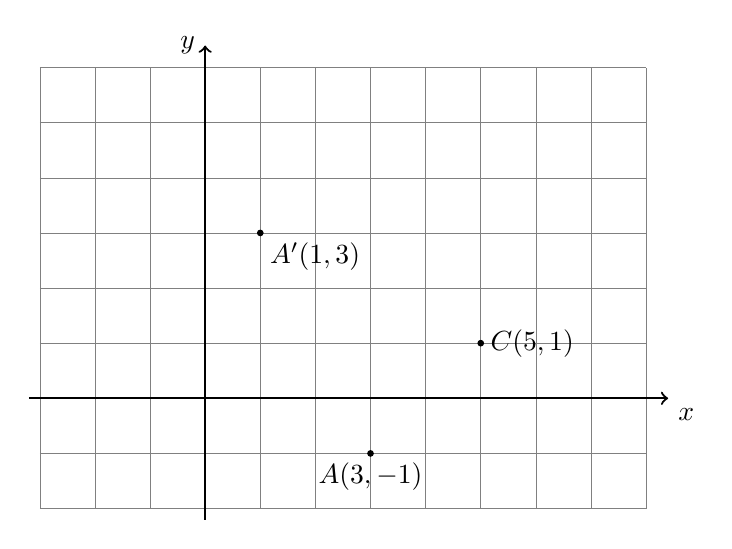
\begin{tikzpicture}[scale=0.7]
      \draw [help lines] (-3,-2) grid (8,6);
      \draw [thick, ->] (-3.2,0) -- (8.4,0) node [below right] {$x$};
      \draw [thick, ->] (0,-2.2)--(0,6.4) node [left] {$y$};
      \draw [fill] (3,-1) circle [radius=0.05] node[below] {$A(3,-1)$};
      \draw [fill] (1,3) circle [radius=0.05] node[below right] {$A'(1,3)$};
      %\draw [->, dashed] (7,1)--(2,3);
      \draw [fill] (5,1) circle [radius=0.05] node[right] {$C(5,1)$};
    \end{tikzpicture}
    \end{flushright}
\end{multicols}

\newpage
\item Reflect the triangle across the $x$-axis, $\triangle ABC \rightarrow \triangle A'B'C'$. Complete the table of the coordinates and plot and label the image on the grid. \vspace{0.5cm}
\begin{multicols}{2}
  $A(1,2) \rightarrow$ \\[0.7cm]
  $B(1,4) \rightarrow$ \\[0.7cm]
  $C(4,2) \rightarrow$ \\[0.7cm]
    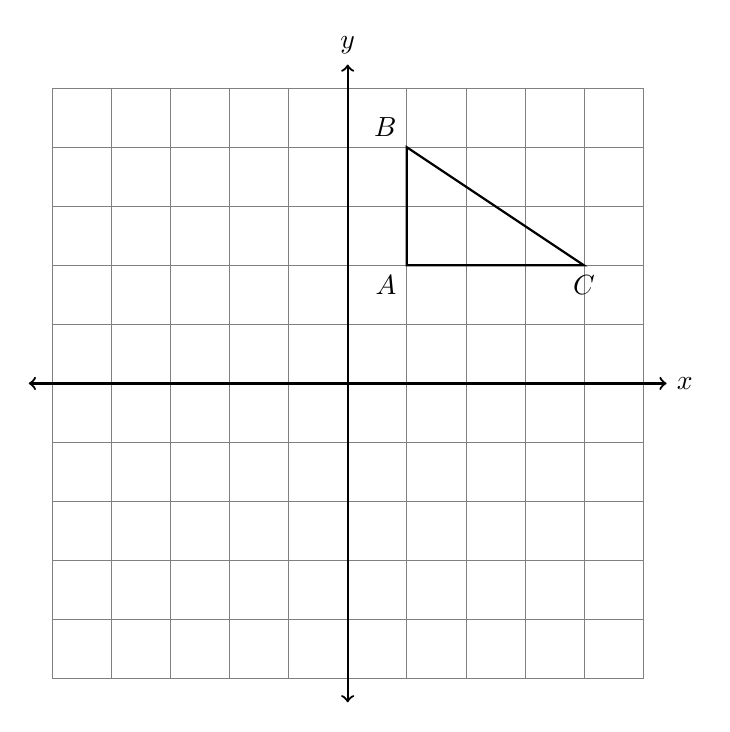
\begin{tikzpicture}[scale=.75]
    \draw [help lines] (-5,-5) grid (5,5);
    \draw [thick, <->] (-5.4,0) -- (5.4,0) node [right] {$x$};
    \draw [thick, <->] (0,-5.4)--(0,5.4) node [above] {$y$};  
    \draw [thick]
      (1,2) node[below left] {$A$}--
      (1,4) node[above left] {$B$}--
      (4,2) node[below] {$C$}--cycle;  
    \end{tikzpicture}
  \end{multicols}

\newpage
\item $\triangle ABC$ is shown with vertices $A(-1,2)$, $B(4,1)$, and $C(6,4)$. Rotate the triangle $90^\circ$ clockwise around the origin. Write down its coordinates in a table and plot and label it on the graph.
  \begin{flushright}
    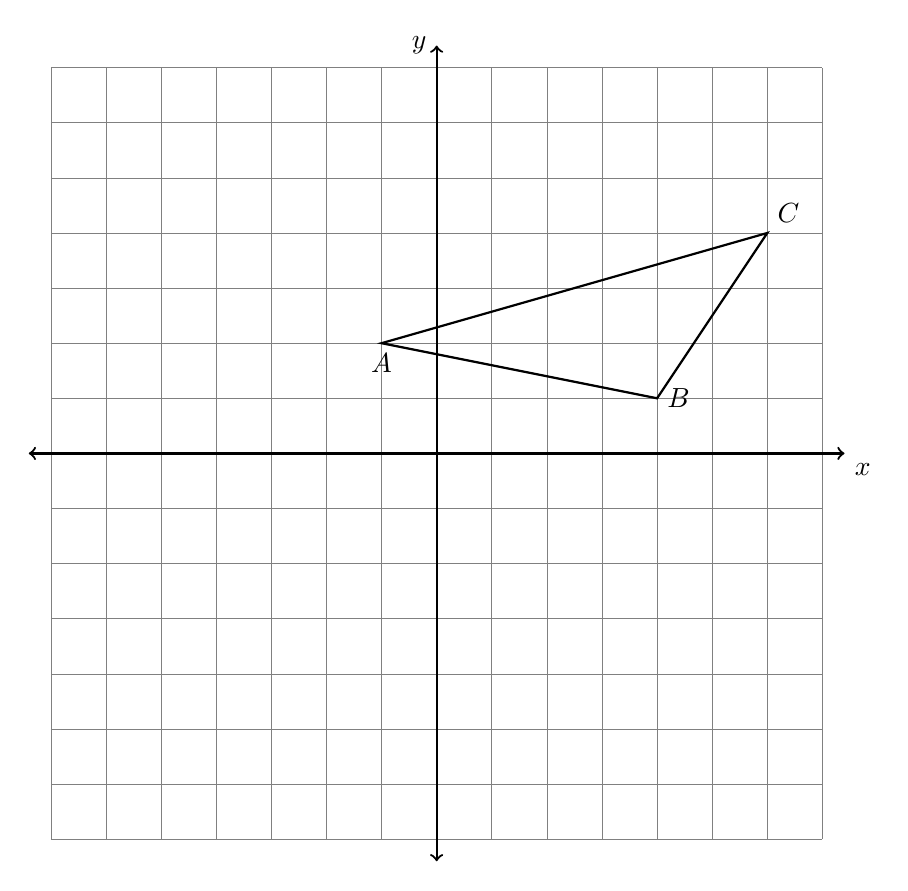
\begin{tikzpicture}[scale=0.7]
      \draw [help lines] (-7,-7) grid (7,7);
      \draw [thick, <->] (-7.4,0) -- (7.4,0) node [below right] {$x$};
      \draw [thick, <->] (0,-7.4)--(0,7.4) node [left] {$y$};
      \draw [thick] (-1,2) node[below] {$A$}--
        (4,1) node[right] {$B$}--
        (6,4) node[above right] {$C$}--
        cycle;
    \end{tikzpicture}
    \end{flushright}


\newpage
\item A dilation centered at $A$ maps $\triangle ABC \rightarrow \triangle ADE$. Given that $BC = 9$, $DE = 15$.
  \begin{enumerate}[itemsep=1.5cm]
    \item Find the value of the scale factor $k$.
    \item Given $AB=12$, find $AD$
    \item Given $AE=12.5$, find $AC$
  \end{enumerate}
    \begin{flushright}
      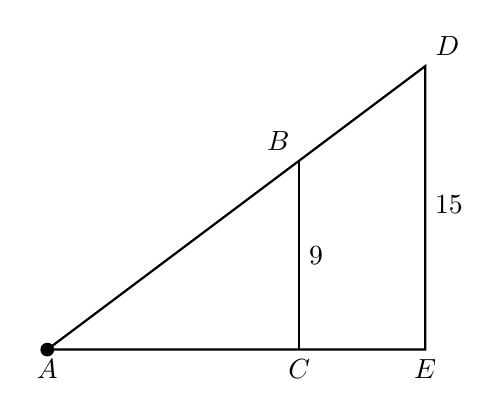
\begin{tikzpicture}[scale=0.8]
        \draw [-, thick] (0,0)--
        (6,0) node[below]{$E$}--
        (6,4.5) node[above right]{$D$}--cycle;
        \draw [thick] (4,0)--(4,3);
        \draw [fill] (0,0) circle [radius=0.1] node[below] {$A$};
        \node at (4,0) [below]{$C$};
        \node at (4,3) [above left]{$B$};
        %\node at (2, 0) [below]{$10$};
        %\node at (2, 2) [above]{$12$};
        \node at (6, 2.3) [right]{$15$};
        \node at (4, 1.5) [right]{$9$};
      \end{tikzpicture}
    \end{flushright}

\newpage
\item Each transformation we study--translation, dilation, rotation, and reflection--have specific details that must be stated to \emph{fully characterize} the transformation. Match the required details with the transformation.
\begin{enumerate}[itemsep=0.5cm]
  \item The center, the degree measure and direction
  \item The line over which it is performed
  \item The horizontal and vertical distances
  \item The center and the scale factor $k$
\end{enumerate}

\newpage
\item A composition of two transformations is applied to $\triangle ABC$, shown in the diagram. Fully characterize the two transformations, in order.
    \begin{flushright}
      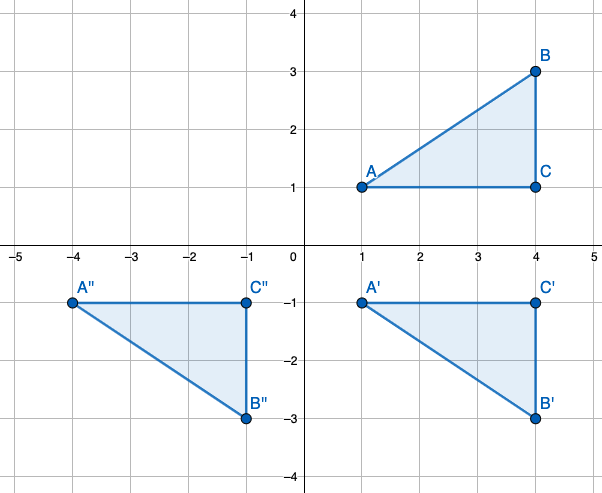
\includegraphics[width=5in]{5-9reflect+translate.png}
    \end{flushright}

\newpage
\item A point labeled $A$ and vector $(-3,1)$ are shown Geogebra/classic. Identify the following objects and tools.
  \begin{enumerate}
    \item Circle the vector
    \item Make an ``X'' where to click for the menu ``Name \& Value'' that will label point $A$ as an ordered pair.
    \item Mark with an arrow the menu where the ``Translate by vector'' tool is found.
  \end{enumerate}
  \begin{flushright}
    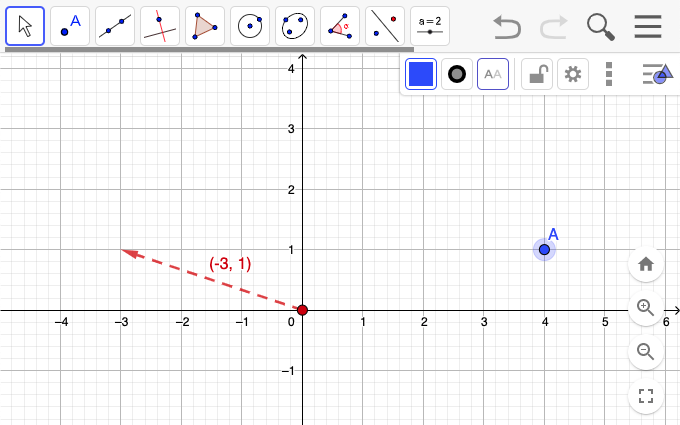
\includegraphics[width=6.25in]{5-9Geogebra_toolbar.png}
  \end{flushright}

\newpage
\item Perform a composition of two transformations using Geogebra/classic. Paste an image of your work in this Classkick slide using the ``camera'' tool.
  \begin{enumerate}
    \item Plot $\triangle ABC$, $A(1,2)$, $B(4,3)$, $C(5,6)$
    \item Mark a point at the origin.
    \item Rotate the triangle $90^\circ$ clockwise around the origin.
    \item Reflect the image $\triangle A'B'C'$ across the $y$-axis.
  \end{enumerate}
    
\end{enumerate}
\end{document}